\documentclass[10pt]{beamer}
\usepackage[brazil]{babel}
\usepackage[utf8]{inputenc}

\usetheme[progressbar=frametitle]{metropolis}
\usepackage{appendixnumberbeamer}

\usepackage{booktabs}
\usepackage[scale=2]{ccicons}

\usepackage{pgfplots}
\usepgfplotslibrary{dateplot}

\usepackage{xspace}
\newcommand{\themename}{\textbf{\textsc{metropolis}}\xspace}

\title{Matemática financeira}
\subtitle{Séries de pagamentos uniformes}
% \date{\today}
\date{}
\author{Prof. Dr. Ricardo Galvão}
\institute{www.rgalvao.com}
% \titlegraphic{\hfill\includegraphics[height=1.5cm]{logo.pdf}}

\begin{document}

\maketitle

\begin{frame}{Conteúdo da apresentação}
  \setbeamertemplate{section in toc}[sections numbered]
  \tableofcontents[hideallsubsections]
\end{frame}

\section{Introdução}

\begin{frame}[fragile]{Séries de pagamentos}

Há vários momentos nos quais necessitamos de grandes volumes de capital. Um bom exemplo é a aquisição de um automóvel, outro exemplo envolve a aquisição de um computador sofisticado. Nessas situações, é comum o indivíduo não possuir todo o capital necessário imediatamente, sendo necessário recorrer a um financiamento em várias parcelas normalmente fixas.\\
O oposto também ocorre. Inúmeras pessoas sabiamente decidem poupar um valor fixo todos os meses com o intuito de deixar a vida muito confortável com o passar do tempo.\\
As séries de pagamentos uniformes servem para auxiliar os indivíduos na realização dos cálculos necessários à consecução de tais objetivos. Ao longo desta apresentação, serão apresentadas as fórmulas e os conceitos de maneira concisa e objetiva.

\end{frame}

\begin{frame}[fragile]{Séries de pagamentos}

Tanto na hora de poupar um quantia fixa todos os meses quanto na hora de tomar um capital emprestado e pagar em parcelas fixas, a matemática financeira serve como instrumento facilitador dessas operações. A seguir, veremos como proceder para calcular o valor das parcelas, o montante a ser tomado ou o valor acumulado no futuro em uma série constante.

\end{frame}


%\section{Tipos de séries}

\begin{frame}[fragile]{Tipos de séries}
Há dois tipos de séries de pagamentos constantes: \\
\begin{itemize}
  \item Séries Postecipadas
  \item Séries Antecipadas
\end{itemize}
\end{frame}

\section{Séries Postecipadas}

\begin{frame}[fragile]{Séries postecipadas}
Nas séries \underline{postecipadas}, o primeiro desembolso (no caso de um empréstimo) ocorre no período seguinte ao valor presente da série. Um bom exemplo é um empréstimo a ser pago em doze parcelas mensais com a primeira parcela vencendo um mês após a contratação.\\
A figura abaixo representa graficamente um fluxo de caixa postecipado com uma entrada de caixa inicial e uma sequência de saídas de caixa constantes.
\begin{figure}
  \begin{center}
    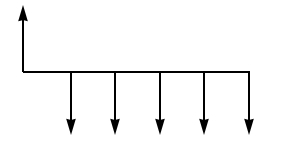
\includegraphics[width=0.5\textwidth]{Fluxopostecipado.jpg}
    \caption{Exemplo gráfico de um fluxo postecipado}
    \label{fig:Fluxopostecipado}
  \end{center}
\end{figure}
\end{frame}

\begin{frame}{Séries postecipadas - Fórmulas}
Nas situações em que não há valores futuros, deve-se utilizar uma das equações a seguir:
  \begin{equation*}
    PV = PMT \left( \frac{ ( 1 + i ) ^{n} - 1 }{ ( 1 + i ) ^{n} . i } \right) 
  \end{equation*}

  \begin{equation*}
    PMT = PV \left( \frac{ ( 1 + i ) ^{n} .i }{ ( 1 + i ) ^{n} - 1 } \right) 
  \end{equation*}

\tiny Onde: \\   PV representa o valor presente \\ PMT representa o valor periódico (parcela) \\ i representa a taxa de juros \\ n representa o número de períodos.
\end{frame}

\begin{frame}{Exemplo de empréstimo em uma série postecipada}
%\twocolumn
\footnotesize  Exemplo: João contraiu um empréstimo no valor de R\$ 6.000,00 com taxa de juros de 2\% ao mês em doze parcelas mensais iguais com a primeira trinta dias após a contratação. Qual o valor da parcela?\\
$ PMT = PV \left( \frac{ ( 1 + i ) ^{n} .i }{ ( 1 + i ) ^{n} - 1 } \right)  $\\
$ PMT = 6000 \left( \frac{ ( 1 + 0,02 ) ^{12} .0,02 }{ ( 1 + 0,02 ) ^{12} - 1 } \right)  $\\
$ PMT = 6000 \left( \frac{ ( 1,02 ) ^{12} .0,02 }{ ( 1,02 ) ^{12} - 1 } \right)  $\\
$ PMT = 6000 \left( \frac{ 1,268242 .0,02 }{ 1,268242 - 1 } \right)  $\\
$ PMT = 6000 \left( \frac{ 0,025365 }{ 0,268242 } \right)  $\\
$ PMT = 6000 . 0,09456  $\\
$ PMT = 567,36  $\\
João deverá pagar doze parcelas iguais de R\$ 567,36.
\end{frame}

\begin{frame}{Séries postecipadas - Fórmulas}
Nas situações onde não há valores presentes, deve-se utilizar uma das equações a seguir:
  \begin{equation*}
    FV = PMT \left( \frac{ ( 1 + i ) ^{n} - 1 }{ i } \right) 
  \end{equation*}

  \begin{equation*}
    PMT =  \frac{ FV.i }{ ( 1 + i ) ^{n} - 1  } 
  \end{equation*}

\tiny Onde: \\   FV representa o valor futuro \\ PMT representa o valor periódico (parcela) \\ i representa a taxa de juros \\ n representa o número de períodos.
\end{frame}

\begin{frame}{Exemplo de poupança em uma série postecipada}
%\twocolumn
\footnotesize  Exemplo: Maria decidiu poupar R\$ 500,00 todos os meses durante oito anos. Considerando uma taxa de juros mensal de 0,6\%, qual o valor acumulado ao final dos oito anos?\\
$ FV = PMT \left( \frac{ ( 1 + i ) ^{n} - 1 }{ i } \right) $\\
$ FV = 500,00 \left( \frac{ ( 1 + 0,006 ) ^{96} - 1 }{ 0,006 } \right) $\\
$ FV = 500,00 \left( \frac{ ( 1,006 ) ^{96} - 1 }{ 0,006 } \right) $\\
$ FV = 500,00 \left( \frac{ 1,775849 - 1 }{ 0,006 } \right) $\\
$ FV = 500,00 \left( \frac{ 0,775849 }{ 0,006 } \right) $\\
$ FV = 500,00 . 129,308244 $\\
$ FV = 64.654,12$\\
Maria deverá acumular um montante de R\$ 64.654,12.
\end{frame}




\section{Séries Antecipadas}


\begin{frame}[fragile]{Séries Antecipadas}
%\onecolumn
Nas séries \underline{antecipadas}, o primeiro desembolso (no caso de um empréstimo) ocorre no momento inicial da série. Um bom exemplo é um empréstimo a ser pago em doze parcelas mensais com a primeira parcela no momento da contratação.\\
A figura abaixo representa graficamente um fluxo de caixa antecipado com uma entrada de caixa inicial e uma sequência de saídas de caixa constantes.
\begin{figure}
  \begin{center}
    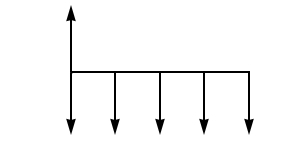
\includegraphics[width=0.5\textwidth]{Fluxoantecipado.jpg}
    \caption{Exemplo gráfico de um fluxo antecipado}
    \label{fig:Fluxoantecipado}
  \end{center}
\end{figure}
\end{frame}


\begin{frame}{Séries antecipadas - Fórmulas}
Nas situações em que não há valores futuros, deve-se utilizar uma das equações a seguir:
  \begin{equation*}
    PV = PMT \left( \frac{ ( 1 + i ) ^{n} - 1 }{ ( 1 + i ) ^{n-1} . i } \right) 
  \end{equation*}

  \begin{equation*}
    PMT = PV \left( \frac{ ( 1 + i ) ^{n-1} .i }{ ( 1 + i ) ^{n} - 1 } \right) 
  \end{equation*}

\tiny Onde: \\   PV representa o valor presente \\ PMT representa o valor periódico (parcela) \\ i representa a taxa de juros \\ n representa o número de períodos.
\end{frame}


\begin{frame}{Exemplo de empréstimo em uma série antecipada}
%\twocolumn
\footnotesize  Exemplo: Alex contraiu um empréstimo no valor de R\$ 6.000,00 com taxa de juros de 2\% ao mês em doze parcelas mensais iguais com a primeira no ato da contratação. Qual o valor da parcela?\\
$ PMT = PV \left( \frac{ ( 1 + i ) ^{n-1} .i }{ ( 1 + i ) ^{n} - 1 } \right)  $\\
$ PMT = 6000 \left( \frac{ ( 1 + 0,02 ) ^{11} .0,02 }{ ( 1 + 0,02 ) ^{12} - 1 } \right)  $\\
$ PMT = 6000 \left( \frac{ ( 1,02 ) ^{11} .0,02 }{ ( 1,02 ) ^{12} - 1 } \right)  $\\
$ PMT = 6000 \left( \frac{ 1,243374 .0,02 }{ 1,268242 - 1 } \right)  $\\
$ PMT = 6000 \left( \frac{ 0,024867 }{ 0,268242 } \right)  $\\
$ PMT = 6000 . 0,092705  $\\
$ PMT = 556,23  $\\
Alex deverá pagar doze parcelas iguais de R\$ 556,23.
\end{frame}


\begin{frame}{Séries antecipadas - Fórmulas}
Nas situações onde não há valores presentes, deve-se utilizar uma das equações a seguir:
  \begin{equation*}
    FV = PMT \left( \frac{ ( 1 + i ) ^{n} - 1 }{ i } \right) . ( 1 + i )
  \end{equation*}

  \begin{equation*}
    PMT =  \frac{ FV.i }{( ( 1 + i ) ^{n} - 1 ). ( 1 + i ) } 
  \end{equation*}

\tiny Onde: \\   FV representa o valor futuro \\ PMT representa o valor periódico (parcela) \\ i representa a taxa de juros \\ n representa o número de períodos.
\end{frame}


\begin{frame}{Exemplo de poupança em uma série antecipada}
%\twocolumn
\footnotesize  Exemplo: Bruna decidiu poupar R\$ 500,00 \textbf{ao final de cada mês} os meses durante oito anos. Considerando uma taxa de juros mensal de 0,6\%, qual o valor acumulado ao final dos oito anos?\\
$ FV = PMT \left( \frac{ ( 1 + i ) ^{n} - 1 }{ i } \right).(1 + i) $\\
$ FV = 500,00 \left( \frac{ ( 1 + 0,006 ) ^{96} - 1 }{ 0,006 } \right). (1 + 0,006) $\\
$ FV = 500,00 \left( \frac{ ( 1,006 ) ^{96} - 1 }{ 0,006 }\right).(1,006) $\\
$ FV = 500,00 \left( \frac{ 1,775849 - 1 }{ 0,006 } \right).1,006 $\\
$ FV = 500,00 \left( \frac{ 0,775849 }{ 0,006 }\right)1,006  $\\
$ FV = 500,00 . 129,308244.1,006 $\\
$ FV = 500,00 . 130,084093 $\\
$ FV = 65.042,05$\\
Bruna deverá acumular um montante de R\$ 65.042,05.
\end{frame}



\section{Conclusão}


\begin{frame}[fragile]{Conclusão e considerações}
Esta breve apresentação teve por objetivo compilar de maneira concisa o que é uma série de pagamentos uniformes e como realizar os referidos cálculos.\\
Trata-se de mais um documento do projeto \textbf{Repositório de código aberto voltado a textos sobre Finanças} do professor Ricardo Galvão, que tem por objetivo disponibilizar livremente materiais nas áreas de investimentos e finanças seguindo a licença Creative Commons Attribution-ShareAlike.


\end{frame}


\begin{frame}{Créditos}

Tanto esta apresentação quanto o tema utilizado estão sob a licença  \href{http://creativecommons.org/licenses/by-sa/4.0/}{Creative Commons
  Attribution-ShareAlike 4.0 International License}.
  \begin{center}\ccbysa\end{center}

A apostila pode ser obtida no endereço:
\begin{center}\url{github.com/rcgalvao/financas}\end{center}

O tema pode ser obtido no endereço: 
\begin{center}\url{github.com/matze/mtheme}\end{center}

\end{frame}


\end{document}
